%\documentclass[JIP,draft]{ipsj}
\documentclass[JIP]{ipsj}

%\usepackage[dvips]{graphicx}
\usepackage[pdftex]{graphicx}
\usepackage{latexsym}

\def\Underline{\setbox0\hbox\bgroup\let\\\endUnderline}
\def\endUnderline{\vphantom{y}\egroup\smash{\underline{\box0}}\\}
\def\|{\verb|}

\setcounter{volume}{22}% vol20=2012
\setcounter{number}{4}% 1, 2, 3, 4
\setcounter{page}{100}

\received{2013}{11}{30}
%\rereceived{2011}{10}{1}   % optional
%\rerereceived{2011}{10}{31} % optional
\accepted{2014}{6}{18}

\usepackage[varg]{txfonts}%%!!
\makeatletter%
\input{ot1txtt.fd}
\makeatother%

\usepackage{graphicx}
\usepackage[export]{adjustbox}

\begin{document}

\title{Perception of Trustfulness in Japan's Election}

\affiliate{Waseda}{Global Information and Telecommunication Studies, Waseda University}

\author{Achmad Rully}{Waseda}[arully@computer.org]
\author{Hidenori Nakazato}{Waseda}[nakazato@waseda.jp]


\begin{abstract}
Election is based on trust. Trust.



Election is an essential tool in democracy, and with the advancement of information technology nowadays, all aspects of election quality have also been greatly enhanced. Nevertheless, the quality from the trust aspect is still a distant goal especially in the developing world where the bond of trust between each stakeholder of the society is not as strong as in a developed country. Thus, it is also vital to understand the election from various aspects with the aim to improve it. This paper proposes a tool to understand the risk on an election result by approaching from a risk model of election result handling and simulating the model using a multi-agent simulation.
\end{abstract}

\begin{keyword}
Election Result Risk, Multi-Agent Simulation, Trustworthiness
\end{keyword}

\maketitle

%1
\section{Introduction}
Trust is an essential requirement of an election which is one of the tool in a democracy.

Election is one of essential tools in a democracy. There cannot be a functioning democracy without a functioning election, and vice versa. In social science, election has been researched extensively \cite{Manan2010}.

One thing to be sure is democracy cannot survive without a free and fair election. To hold a free and fair election, transparency and accountability are the keys especially in verifying all aspects of the election. Election is a very laborious process with participation of many entities that have different interests, thus sometimes makes election process a long time. The progress will take longer if problems like a dispute arise, especially if the problems involve some entities who are election stakeholders. Therefore, lately information technology (IT) is used to reduce and minimize the risk in an election. Furthermore, in some cases, utilizing a full end-to-end election process using IT. Nevertheless, the use of IT also has its own risks as described in \cite{Neumann1995}.

The election process is a cumbersome and complicated process that usually involves each citizen of a country, it starts from the ratification of the election law that is agreed upon virtually by all stakeholders, and ends with the declaration of the election result with the endorsement of legitimate candidates. There is no all-in-one solution to handle it as the process is also different in each country, some countries also change the election law for each election. \Figref{fig:ecomplex} shows the complexity of the election process in Indonesia's 2009 election as a process that involved around 519.920 poll stations around the country with 172 million people, with a logistic movement from the Central Election Commission in the top to each poll station in the bottom and back to the top after Election Day with a total cost to reach around US\$850 milion.

Our approach is to focus on one of the main risks in an election, which is the handling of the election result starting from the end of the election day to submit votes until the declaration of the final result. We developed a model of election result risk to better understand how the process and the interaction between each stakeholder after election day can influence the trustability of the election and in particular the trustability of each poll station. Our model then was put on a multi-agent simulation to simulate the election in Indonesia in 2009 and show the comparability of the result with what happened in the election in 2009.

In the model, each stakeholder's parameter can be adjusted to reflect the society in which the election is going on. Thus, with the model we can predict how the election will proceed in terms of trustworthiness and will help in understanding risk in the election process. The model can also be used to predict the usability of a proposal for a change or a proposal for an added tool in an election.

\begin{figure}[tb]%1
\setbox0\vbox{\it
  \hbox{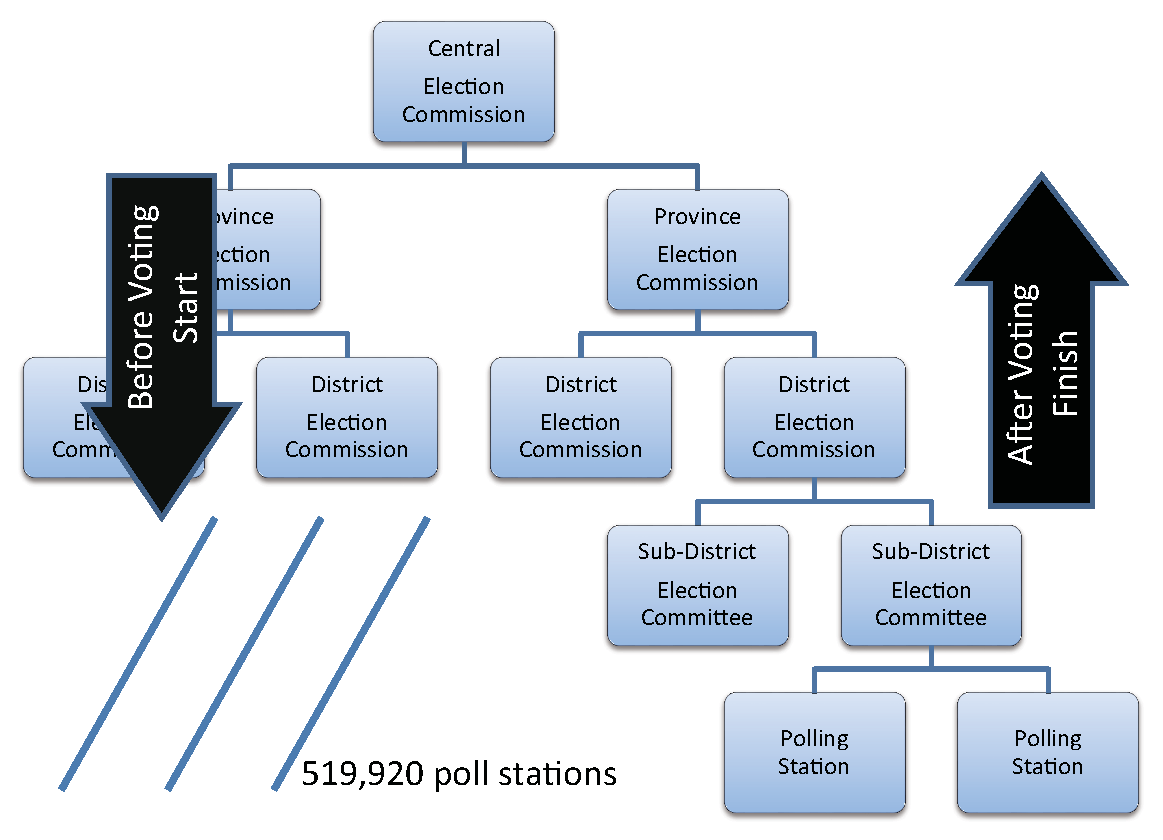
\includegraphics[scale=0.4]{images/ElectionComplexity.eps}}}
\centerline{\fbox{\box0}}
\caption{Election Process}
\label{fig:ecomplex}
\end{figure}

%2
\section{Background}

Here we will discuss about why we need to create a risk model of election result handling.

\subsection{Election Process}%2.1
\label{ElectionProcess}

Election especially national election is a complex process, but in general there are 6 election stages:

\begin{enumerate}%{
\item \|Pre-preparation|.\\
In this stage, the parliament prepares a legal framework for an election by passing a law. The law enlists about how the candidate will be decided, how many ballots for a ticket/seat, how many electorates per area, etc. Parliament and head of state together will then choose who will be the commissioners in the central election committee including how much budget is needed for the election.

\item \|Preparation|.\\
In this stage, the chosen commissioners with bureaucrats in the central election commission will prepare the technical details of the election based on the law. Lately, as the election is getting more complicated, IT has been in use to handle some processes like candidates registrations, tabulation etc. \cite{Budi2008}.

The election commission prepares all logistics for the election like ballots, ballot boxes, even pens to write in manual voting. For electronic voting, the commission is required to prepare eVoting machine and check its readiness. The commission also needs to prepare their bureaucrats readiness to the law and needs to socialize technical details to all election stakeholders.

After the preparation in the commission is complete, all election logistics needs to be transported and distributed to every province election commissions, then to district election commissions. After that the committees will coordinate each technical detail and the distribution of logistics to every poll station under their jurisdiction.

\item \|Election|.\\
In the Election Day, officers are ready in every poll station; registered electorates go to their registered poll station to cast their ballot. Before electorates can vote, they must bring their IDs, and the officers will compare the ID with the list of registered electorate. Besides officers from election committees, there are also witnesses from every available party. However because not every party can afford to send their witnesses to every poll station, not every poll station has all witnesses from every party. Some poll stations also do not have any witnesses; therefore electorates could volunteer to be witness. The election usually takes one day on the same date for every place, but because of geographical challenge etc., some areas get exceptions.

After voting time is up, the ballot box is opened, and the counting begins in every poll station. The tally result will then be declared in the poll station, with all available witnesses from political parties and electorates singing the official tally result on the poll station. After that, all ballots are put in ballot boxes and sealed, and together with the result, they are sent to its sub-district election committee.

\item \|Result Reporting and Verification|.\\
The election committee in sub-district tallies the result with other poll station results under the committee, and the total result is sent to the district election commission. The result then goes to the province election commission who tallies and sends the combined result to the central election commission. The tally result in each step is open to public, so each party can get the result and compare it with its own tally result, along with the progress of gathering and tallying all the results from each province's election commission by the central election commission. The ballot papers inside the ballot boxes are stored by the sub-district's election committee in a sealed condition. Usually, in every step there would be police present.

\item \|Dispute Resolution|.\\
In this stage, a party or electorate can petition a protest if they found irregularities by bringing witness or proof. Beside money politics and other type of cases, some of the cases that usually aroused which related to this proposed system were: a result discrepancy between a party's own tally result in a sub-district, a district or a province with the tally result in sub-district, district or province; a data mismatch because of an error in inputting a tally result from each poll station, a sub-district or a district. To solve the disputes, the court in some cases had to open the ballot boxes and manually count the vote from each ballot paper. If the ballot boxes are in a remote area, the cost in time and money will be high.

\item \|Final Result|.\\
In this stage, after the Supreme Court decides every dispute, the final outcome can be announced. If there are a lot of cases that take time and money, then the announcement of the final election result will need to be postponed, or the Supreme Court will proceed in announcing the final result by ignoring some costly cases
\end{enumerate}%}


From stages 1 to 2, almost every aspect is a political aspect like the requirement of a candidate, the registration, etc, therefore they are out of scope of this paper. The complexity and problems in stages 1 to 2 usually can be handled using election information systems based on IT. This paper focuses on stages 3 to 4, where the risk is high and the complexities of the problems usually focus on ensuring the election result is not tampered.

%\newpage

\subsection{Related Work}%2.2

As the focus of election research in ICT field is on eVoting \cite{Bryans2006}\cite{Volkamer2007}\cite{Mercuri2004}\cite{Kremer2005}, more countries research, try and implement it \cite{Tiresias20121212}. They argue that eVoting machine can lower the risk of cheating and can make perceived trustworthiness higher. Nevertheless, some say eVoting also has shortcomings \cite{ Hisamitsu2007}\cite{ Schryen2009} because in regard to risk some implementation did not address more important problems in elections \cite{ Wolchok2010}.

Some researchers develop a model to understand the election like \cite{ Yoneyama2007} but their focus are on voters mind and decision, and not on the trustworthiness of an election. Others develop a model for a theoretical election like \cite{ Rivest2008}\cite{ Langer2009}\cite{ Ryan2009}.

On the other hand, multi-agent simulation has gained attention lately as a tool to understand the human behavior \cite{ Drogoul2013}. Election is born because of human interaction and to understand it we need to use tools that simulate human behavior as similarly as possible.



%3
\section{Election Result Risk Model}

We discuss here about how we developed the election result risk model.

\subsection{Approach}%3.1

As we analyzed election process as described in subsection \ref{ElectionProcess}, in this paper we focused on the election process that starts from the start of election day in which the voters put their votes in the ballot box, and stop until the election result is decided lawfully. We found out that the process pattern is somehow similar between elections, whether in an election in a developed country or in a developing country.

In an idealistic environment, after the time is up for voters to put their votes in a particular poll station, the process pattern is started with opening the ballot box to count the votes by one or more officials in attendance of one or more party witnesses and observers. Officials are persons that are authorized by the central authority to manage a particular poll station. Party witnesses are persons that are authorized by parties (or candidate's supporter groups if the candidate is independent) participating in the election to witness the election process in a particular poll station. Observers are persons that are not in any official duty related to the election, whether it is voters themselves or observers sent by election monitor organizations. The whole process is guarded by one or more security officials usually police officers. At the end of the count process, the particular poll station will have a tally result which is a recapitulation of all votes in the particular poll station.

In this stage, the risk of tampering with the tally result is high because officials have the whole access to the ballot box and the resulting tally result. The risk is higher when others like party witnesses, observers or police officers do not attend the counting process. The absence of others will impact the behavior of officials negatively. In a country where the police is not independent and under the influence of one of the election stakeholders, the possibility of the police also involving in the tampering with the result directly is also high.

The tally result then will be brought to the second stage of the election hierarchy in a particular area to be counted with other poll stations' tally results in the same area. The sealed ballot box with the voter's vote inside it will be moved to a secure location. Guarding the whole process is one or more police officers.

In this stage, the risk of tampering with the tally result is high because police officers and officials have the whole access to the tally result. Police officers guarding the tally result could possibly switch the ballot box and the tally result especially in a remote area. The officers could also participate in changing the tally result. The officers could independently change the tally result with the assumption that nobody will check the sealed ballot box or because no one else in the particular poll station will reliably verify the second stage tally result in a particular area.

If the counting process in the second stage of election hierarchy is finished with the declaration of the second stage tally result in the particular area, the tally result will be brought to the third stage, the fourth stage and so on according to the election hierarchy to facilitate the recapitulation of counting results in the same hierarchy.

After we reviewed the process described above, we found out that the most important entity to be considered as important value is the trustworthiness value of a particular poll station. A poll station has a very distinct role, because it is the first and the last time every stakeholder of the election like a voter, a party official, an election official, a police, meet in person as a stakeholder role. Humans tend to value meeting in person as a strong point to prevent unethical behavior \cite{Nogami2009}. The value of trustworthiness in each poll station will determine the risk of tampering the whole election result. Therefore, we decide to designate the trustworthiness of election result in a particular poll station as a benchmark to analyze the whole election.


\subsection{The Risk Model}%3.2
%parameter, process, actors, interaction, etc

%table for model's parameters
\begin{table}[tb]
\caption{Agent \& Parameter}
\label{tab:modpar}
\hbox to\hsize{\hfil
\begin{tabular}{l|cccc}\hline\hline
\quad    &\quad no &\quad\quad\quad ef &ifp& bc\quad\\\hline
\quad op  &\quad O &\quad\quad\quad  O & X & O\quad   \\
\quad pol &\quad O &\quad\quad\quad  O & O & O\quad  \\
\quad pw  &\quad O &\quad\quad\quad  O & O & X\quad   \\
\quad ob  &\quad O &\quad\quad\quad  O & O & X\quad   \\\hline
\multicolumn{4}{l}{op\,: {\tt official}\quad
	pol\,: {\tt police officer}}\\
\multicolumn{4}{l}{pw\,: {\tt party witness}\quad
	ob\,: {\tt observer}}\\
\multicolumn{4}{l}{no\,: {\tt number of agent}\quad
	ef\,: {\tt existential factor}}\\
\multicolumn{4}{l}{ifp\,: {\tt influence factor positive}\quad
	bc\,: {\tt bad conduct}}\\
\end{tabular}\hfil}
\end{table}

\begin{figure*}[t]
\setbox0\vbox{\large
  \hbox{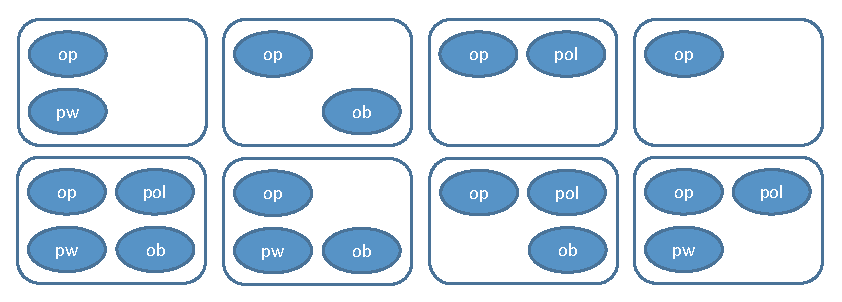
\includegraphics[]{images/agents.eps}}}
\centerline{\fbox{\hbox to.9\textwidth{\hss\box0\hss}}}
\caption{8 possible condition in a poll station}
\label{fig:8posinTPS}
\end{figure*}

Every poll station is usually attended by voters that live around the poll station. Voters that live in the same neighborhood have different levels of trustworthiness to their neighborhood, based on three characteristics: ability, benevolence and integrity \cite{Mayer1995}. Ability is related to a group of skills, competencies and characteristics that enable a person to have influence. Benevolence is the extent to which a person wants to do a good role to others aside from an egocentric profit motive. Integrity is the quality of being honest and fair from a person, that other people expect he or she will adhere to a set of principles.

From these three factors, we derive three parameters for our election risk model: existential factor, influence factor positive and bad conduct. Existential factor (ef) is a person’s benevolence that he or she wants to prove that he has integrity. Influence factor positive (ifp) is an ability of a person to do good to fulfill an adherence to principles. On the contrary, bad conduct (bc) is an ability of a person to break adherence to the principles.

We identified that there are four distinct agents in a particular poll station: official (\textit{op}), police (\textit{pol}), party witness (\textit{pw}) and observer (\textit{ob}). Each one of them has a particular important role related to the outcome of the election result, from the beginning of election day until the sending of poll station tally result to the second stage. In each poll station there are eight possibilities of \textit{op}, \textit{pol}, \textit{pw} and \textit{ob} existence as shown in \figref{fig:8posinTPS}. The possibilities represent the interaction and influence of each actor. The model should reflect all the possibilities.

As a unit to measure the risk on a tally result in regard to the interaction and influence between agents, we define \textit{T} as trustworthiness. Each \textit{T} will be attached to the tally result from each particular poll station. \textit{T} has value \|[0,100]|\ where a value of 0 means there is no trust and a value of 100 means complete trust. Note that “no trust” is not equivalent to “bad result” in front of the law, but it means that the tally result from a particular poll station does not meet the criteria for trust. There was evidence in court about election that people was sentenced with tampering the tally result but the court still uphold the result. The value of $T$ will depend on the existence of agents and the interaction between each agent. The existence factor will build up an inital value of $T$, and the interaction will make the $T$ value up or down.

Trustworthiness in an election context is a value of trust that voters give to the election so that the election will be trustworthy. When one or more parts in an election do not behave in accordance to the expected behavior, then the risk that trustworthiness is decreasing is higher. In this model, trustworthiness is a value of trust that voters give to each tally result, in which the value will change according to the behavior of the official, the police, the party witness and the observer.

The model has parameters as shown in \tabref{tab:modpar}. In a real election, it is not always the case that each category of agent is present in a particular poll station, so the model reflects the real condition by also having a number of agents in an election as a parameter. At the beginning of the election day, the value of \textit{T} will depend on the existence of each category of agent (\textit{op}, \textit{pol}, \textit{pw} and \textit{ob}) in a particular poll station. For a poll station that has all categories of agents, we can put the initial \textit{T} at 100 as a total value of agents' \textit{ef}. In an ideal condition, agent \textit{op} has the biggest \textit{ef} value compared to others as he is the one who has the authority to manage the poll station. In a place that the bond between stakeholders is low like in a failed country, it is possible that \textit{op}'s value of \textit{ef} is lower than others.

After the start of counting votes, the presence of \textit{pol}, \textit{pw} and \textit{ob} possibly can influence the behavior of \textit{op} positively (we called this parameter as \textit{ifp}). Thus, \textit{ifp} value from each category of agent will add up to \textit{T}. The \textit{ifp} value for each agent is not fixed as each agent in the real life has different behavior (therefore, a different \textit{ifp} value) even in the same category. 

On the other hand, \textit{op} and \textit{pol} are entities that have a direct access to the tally result so each has a value of bad conduct (as \textit{bc}) that possibly can tamper with the result. Therefore, a \textit{bc} value from \textit{op} and \textit{pol} will negate \textit{T} accordingly. The \textit{bc} value for each agent is also not fixed as each agent has a different behavior.

In simulation, we can define a maximum and minimum value for \textit{ifp} and \textit{bc} for each agent to reflect the society where the election is happening, and then the simulation platform will designate it randomly.

In the second stage and beyond, agents that exist are \textit{op} and \textit{pol}, although there is no \textit{ef} value in here because we observed from the real election that in the second stage and beyond it is certain that the official and the police are present. The reason for this is because the number of places for the second stage process is also considerably lower compared to the number of poll stations, and the place is also not as remote as in all poll stations. In the 2009 election in Indonesia, there were 519,920 poll stations with the number of sub-districts at around 5,200 \cite{KPU200903}\cite{PemiluIndonesia20090313}. There is also no value of \textit{ifp} because each \textit{op} and \textit{pol} doesn't receive influence from others agents, but each can tamper with the result. Therefore, \textit{op} and \textit{pol} have their own \textit{bc} that will negate \textit{T} accordingly.


%4
\section{Simulation}
%isi: setup GAMA; 
\subsection{Simulation Platform: GAMA}

There are a number of simulation platforms that can do multi-agent simulations, but among them we choose GAMA. GAMA is a simulation platform, which aims at providing field experts, modeler, and computer scientists with a complete modeling and simulation development environment for building spatially explicit multi-agent simulations \cite{GAMAplatform}. It has been in development since 2007.

GAMA platform was chosen in this paper because it has:
\begin{enumerate}%{
\item Ability to handle a vast number of heterogeneous agents.\\
We need a powerful platform that can handle a lot of agents where each has a different role, as elections have a lot of poll stations which also have agents interacting inside them. The platform can provide this capability without a need for a big server.

\item Library of primitives (agent's movement and interaction, mathematical function, etc.) that are large and extensible.\\
Platforms that can provide a useful library will surely shorten the time to deploy the model. GAMA is one of the platforms that we compared, that we did not need to create our own library to deploy the model.

\item Ability for automated controlled experiments by automatically changing parameters.\\
GAMA provides ways to change simulation parameters like manual, automatic random, in-simulation parameter change etc. This capability will help to analyze the simulation result. The capability can also be useful when we want to show the simulation to other people who are not expert in computers.

\item Familiar environment.\\
GAMA is based on JAVA language, so the GAML (GAMA simulation syntax) is similar with JAVA language although not the same. Its user interface is also based on the Eclipse platform with seamless integration between the editor, the compiler and the simulator.
\end{enumerate}%}

The platform has still been undergoing a lot of development because when we were deploying the model to the platform, there were new versions that fixed some bugs but also introduced some change to the GAML language. Fortunately, the change was backward compatible so there was no need to change a lot of things.


\subsection{Simulation Setup}%4.1

Using the GAMA platform, we created and defined one template of agent who represents the tally result in a particular poll station. We also created and defined four other templates of agents as in \figref{fig:8posinTPS}, which is official \textit{op}, security officer or police \textit{pol}, party witness \textit{pw} and observer \textit{ob}. GAMA will populate the templates according to the number of agents (parameter \textit{no}) that we want. The number of agents who represent the tally result in a particular poll station is the same with \textit{op}’s \textit{no}.

Each agent carries parameters (\textit{ef}, \textit{ifp} and \textit{bc}) accordingly as shown in \tabref{tab:modpar}. Parameters \textit{ef} is a fixed value, whereas parameters \textit{ifp} and \textit{bc} is a maximum value that GAMA will randomly set for each agent.

In simulation initialization, each agent in the same poll station contributes its \textit{ef} to the agent who represents the tally result in a poll station as initial \textit{T}. After initialization, as the simulation time goes by, \textit{op} and \textit{pol} will decrease \textit{T} randomly, and \textit{pol}, \textit{pw} and \textit{ob}’s \textit{ifp} will increase \textit{T} randomly. After some fixed simulation time, the interaction stops with \textit{T} as the tally result representation in a particular poll station has been settled.

The agent who represents the tally result in a poll station will carry the \textit{T} to the second stage. In the next stage, as is the real election, only \textit{op} and \textit{pol} are present. Thus, \textit{op} and \textit{pol}’s \textit{bc} will decrease \textit{T} randomly and \textit{pol}’s \textit{ifp} will increase \textit{T} randomly. After some fixed simulation time, the interaction stops as a representation that is the recapitulation of tally results in the same hierarchy is finished.

Next, the agent who represents the tally result in a poll station will carry the \textit{T} to the next stage, and the similar interaction as in the second stage happens, and after some fixed simulation time the interaction stops.

The \textit{T} from the agent who represents the tally result represents the trustworthiness of a particular poll station.


\subsection{Simulation Parameters}%4.2

%simulation parameters
\begin{table}[tb]
\caption{Simulation Parameters}
\label{tab:simpar}
\hbox to\hsize{\hfil
\begin{tabular}{l|cccc}\hline\hline
    &  no  & ef & ifp & bc\\\hline
op  & 5199 & 50 & -   & 3   \\
pol & 4200 & 20 & 7  & 10  \\
pw  & 3200 & 20 & 5   & -   \\
ob  & 2200 & 10 & 3   & -   \\\hline
\multicolumn{4}{l}{op\,: {\tt official}\quad
	pol\,: {\tt police officer}}\\
\multicolumn{4}{l}{pw\,: {\tt party witness}\quad
	ob\,: {\tt observer}}\\
\end{tabular}\hfil}
\end{table}

We deployed the model to the GAMA platform using parameters as shown in table \tabref{tab:simpar}. We put the parameters as similarly as possible with Indonesia's election in 2009 \cite{KPU200903}\cite{PemiluIndonesia20090313}.

In the 2009 election, there were 519,920 poll stations, and in the simulation we take sample of 1\% of all poll stations. We found out that the result in the order of 100.000 should not be very different with the order of 1.000, so instead of 519,920 we put the number of poll stations in the simulation to 5.199. Accordingly, the number of official agents were 5.199. There was no exact number of police officers, party witnesses and observers attending poll stations in 2009 election, so we predicted the parameters based on an estimation from data that the authority and newspaper had provided.

To help in determining \textit{ef} value, we made a survey of Indonesian voters' perception of Indonesia Election 2009\cite{SurveiPersepsiPemilu2009}. The result are around 75 respondents responded with 71 valid response. From valid response with maximum value of 3.00, voters give average value of the role of official as 2.41, security officer as 2.31, party witness as 2.34 and observer as 2.03. This perception is in line with our perception.

Thus, we put \textit{op}'s \textit{ef} to 50 because \textit{op} was authorized from the election authority, and usually poll station's official consisted of some community's figures around a particular poll station. Regarding \textit{pol} and \textit{pw}'s \textit{ef}, we put it at the same 20 because in a particular poll station, the presence of each of them had a big effect to the whole trustworthiness of the poll station although not as big as poll station officials. We put the same number of \textit{ef} because voters perception of the role of both of them are similar (2.31 and 2.34 respectively). For \textit{ob}'s \textit{ef}, we only put 10 because the presence of \textit{ob} in a poll station had no impact as big as \textit{op}, \textit{pol} or \textit{pw}. If all agents were present in a poll station, the initial trustworthiness \textit{T} would be 100, but if only \textit{op} was present in a poll station then the initial trustworthiness would be 50.

Regarding \textit{ifp}, we put \textit{pol} at 7 because the watchful eye of police could influence officials to do their jobs according to the law. \textit{pw} also had big influence though not so big as police's influence, so that we put it at 5. \textit{ob} had a small influence with 3. To mimic the real situation in which everyone even in the same category was different, we randomized the \textit{ifp} value for each category of agent in each poll station.

For \textit{bc}, we put \textit{op}'s \textit{bc} to 3 because we believed they would try to hold on their reputation as figures in their locality to act according to the law, but for \textit{pol} we put it at 10 because the police accountability and transparency was not as clear as official. In Indonesia, the police is under the jurisdiction of the President which belong to a particular political party.


\subsection{Simulation Reliability}%4.3

\begin{figure}[tb]%1
\setbox0\vbox{\it
  \hbox{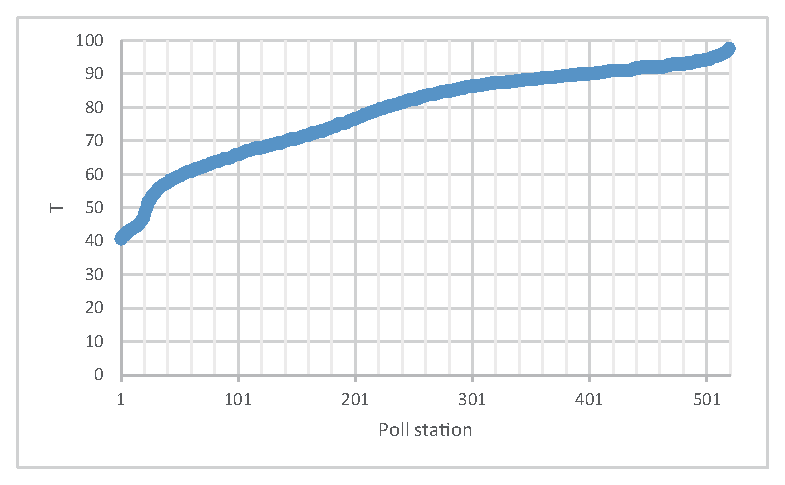
\includegraphics[scale=0.6]{images/graph-sampling100.eps}}}
\centerline{\fbox{\box0}}
\caption{10 sampling of 0.1\% TPS}
\label{fig:sampling100}
\end{figure}

\begin{figure}[tb]%1
\setbox0\vbox{\it
  \hbox{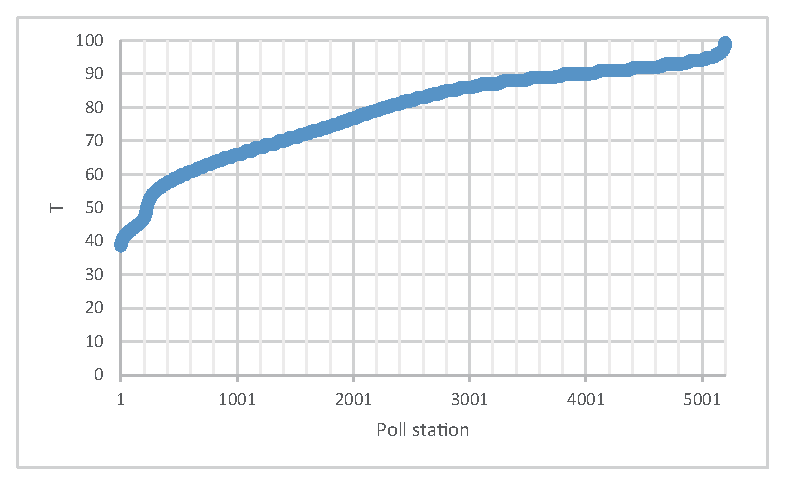
\includegraphics[scale=0.6]{images/graph-sampling1k.eps}}}
\centerline{\fbox{\box0}}
\caption{10 sampling of 1\% TPS}
\label{fig:sampling1k}
\end{figure}


As we don't simulate all the poll station (in the order of 519,920) and instead only a sample of the poll station, we will show that the result is not different. To prove our point, we run 10 times simulation of 0.1\% of poll stations and 10 times simulation of 1\% of poll stations. The average result are shown in two graphs.

\figref{fig:sampling1k} shows the result of 10 samples of simulation of 1\% of poll stations and \figref{fig:sampling100} shows the result of 10 samples of simulation of 0.1\% of poll stations. Both graph are quite similar even though \figref{fig:sampling1k} has 5,199 poll stations and \figref{fig:sampling100} has 520 poll stations. This result shows that the multi-agent simulation can produce the same result event though we take only a sample of all poll stations. Certainly, if we simulate more poll stations then the graph will be more smooth.


\subsection{Result}%4.4

\begin{figure}[tb]%1
\setbox0\vbox{\it
  \hbox{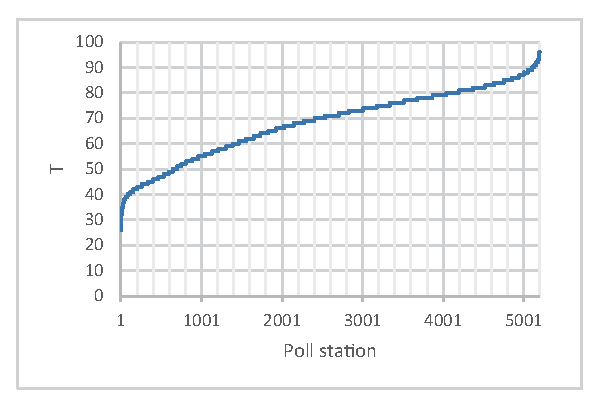
\includegraphics[scale=0.8]{images/Trustworthiness1.eps}}}
\centerline{\fbox{\box0}}
\caption{Trustworthiness of 2009 Indonesia election}
\label{fig:result1}
\end{figure}

\begin{figure}[tb]%2
\setbox0\vbox{\it
  \hbox{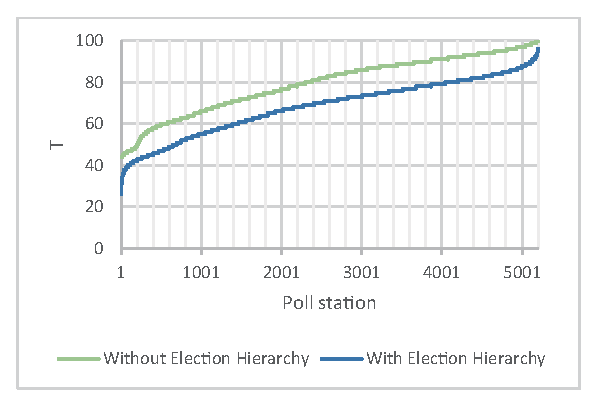
\includegraphics[scale=0.8]{images/Trustworthiness2.eps}}}
\centerline{\fbox{\box0}}
\caption{Trustworthiness of 2009 Indonesia election\\
compare with other method}
\label{fig:result2}
\end{figure}

\begin{figure}[tb]%3
\setbox0\vbox{\it
  \hbox{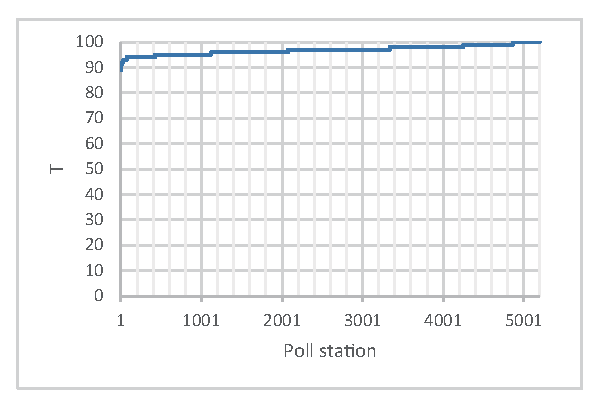
\includegraphics[scale=0.8]{images/Trustworthiness3.eps}}}
\centerline{\fbox{\box0}}
\caption{Trustworthiness of hypothetical election}
\label{fig:result3}
\end{figure}

According to the simulation, the trustworthiness of Indonesia's 2009 election based on 5.199 poll stations is shown in in \figref{fig:result1}. Around 75 poll stations or 7.500 poll stations in the real election has \textit{T} below 40. This is comparable to the number of poll stations in 2009 election in which its tally result was questioned in the Constitutional Supreme Court. \cite{kemitraan201109}. The mean value of \textit{T} is around 68, which is not high though not very low, which means the perceived trustworthiness of the election is not high. The low value of election trustworthiness means that the risk in election result handling process is high. In Indonesia's 2009 parliamentary election, the election itself was deemed successful, but the final result announcement was dragged for more than one month and the final result was finally decided by the Constitutional Supreme Court and not by the central election committee. This happened despite a heavy use of IT to handle the election result.

We also made another simulation using the same parameters. In this scenario, suppose we propose a radical election process change by implementing a system that somehow has a device that can send the tally result from each poll station directly to the central election committee to be recapitulated. When the change is implemented, the tally result from each poll station will bypass all processes in stages, consequently eliminating the possibility of bad conduct by officials and the police.

The resulting graph is shown in \figref{fig:result2}. In this scenario, the number of poll stations in which its tally result was questioned should be nil as no poll station has \textit{T} value below 40. The value of \textit{T} as a whole also up, although the perceived trustworthiness is not in a high bar as the mean value of \textit{T} is 79. This low value happens because the initial trustworthiness of some poll stations are low and the bad conduct factor is quite large especially for the police officers.

In \figref{fig:result3} we show how the model behave when we changed the parameters: the number of agent \textit{pol}, \textit{pw} and \textit{ob} is the same with the number poll stations; and the pol's value of bc is 3 (and not 10). As the mean value of T is around 96, the risk is low because of the participation from all the stakeholders combined with the good behavior of police officers.


%5
\section{Conclusion and Future Work}

This paper presents a risk model in handling the election result from a polling station until a final result ratification using the trustworthiness value to gauge the risk. The model can be used to better understand how to evaluate and improve an election result process. Various variables in a real election were observed and then incorporated to the proposed model. Using a multi-agent simulation we can examine the model usefulness and predict how the risk in an election will be when we change the process.

We intend to develop the model further in the future, to adapt with more conditions. In the current model, we understand that to achieve a lowest risk we need to depend on the presence of all the stakeholders in poll stations. In a developed country, the virtual perceived trustworthiness of election is high although the participation of citizens in the election is very low. We called it virtual because a real good election should attract all the stakeholders.

In relation to determining parameters, in the future we intend to work with a social science researcher to make a survey scientifically and incorporate the result to the simulation.

Based on the enlightenment from developing the model, there are a number of researches we want to pursue in the future. One of the researches is a study on new election result handling system.


%\bibliography{mybib}{}
\bibliography{BIB/rully_bib}{}
\bibliographystyle{ipsjunsrt-e}

\begin{biography}

%\profile{Achmad Rully}{-\@.}
\profile{Achmad Rully}{received B.E. degree in information from Keio University in 2000 and M.E. in information and telecommunication from Waseda University in 2003. He is currently pursuing Ph.D. with Waseda University.\\
His current research interests include election, security, privacy and trust. He is a member of IEEE and a student member of ACM and IPSJ.
}
%
%\profile{Hidenori Nakazato}{-\@.} 
\profile{Hidenori Nakazato}{received B. Engineering degree in electronics and telecommunications from Waseda University in 1982 and MS and Ph.D. degrees in computer science from University of Illinois in 1989 and 1993, respectively.  He was with Oki Electric from 1982 to 2000.  Since 2000, he has been a faculty member at Waseda University, Japan. His research interests include performance issues in distributed systems and networks. He is a member of IEEE, ACM, IEICE and IPSJ.\\
He served as the editor of IEICE Transactions on Communications from 1999 to 2002. He is the Chair of IEICE Communications Society Editorial Board.  He also served as an executive committee member of IEEE Region 10 from 2009-2010 and 2013-2014, and is serving as a member of several IEEE Member and Geographic Activity committees since 2010.
} 
%
%
\end{biography}
\end{document}
